
\documentclass[12pt]{article}
\usepackage{graphicx}
\usepackage{booktabs}
\usepackage{geometry}
\geometry{margin=1in}
\usepackage{amsmath}
\usepackage{float}
\usepackage{hyperref}
\hypersetup{
    colorlinks=true,
    linkcolor=blue,
    filecolor=magenta,
    urlcolor=cyan,
}
\title{Experiment 2: Email Spam or Ham Classification using Naïve Bayes, KNN, and SVM}
\author{Sri Sivasubramaniya Nadar College of Engineering, Chennai\\Department of Computer Science and Engineering\\Academic Year: 2025--2026}
\date{}

\begin{document}
\maketitle

\section*{Aim}
To classify emails as spam or ham using three classification algorithms—Naïve Bayes, K-Nearest Neighbors (KNN), and Support Vector Machine (SVM)—and evaluate their performance using accuracy metrics and K-Fold cross-validation.

\section*{Objective}
\begin{itemize}
  \item Load and preprocess the dataset.
  \item Visualize and understand the distribution of features and target classes.
  \item Apply Gaussian, Multinomial, and Bernoulli Naïve Bayes classifiers.
  \item Evaluate KNN for various $k$ values and algorithms (KDTree and BallTree).
  \item Compare SVM with linear, polynomial, RBF, and sigmoid kernels.
  \item Use GridSearchCV to find optimal hyperparameters.
  \item Evaluate all models using accuracy, precision, recall, F1-score, AUC, and confusion matrix.
  \item Perform 5-Fold cross-validation and summarize the findings.
\end{itemize}

\section*{Libraries Used}
\begin{itemize}
  \item pandas, numpy, matplotlib.pyplot, seaborn
  \item sklearn.model\_selection, sklearn.metrics
  \item sklearn.naive\_bayes, sklearn.neighbors, sklearn.svm
\end{itemize}

\section*{Dataset}
The dataset used is the \textbf{Spambase} dataset from Kaggle, containing email features extracted and labeled as spam or ham.

\section*{Code : }
\begin{verbatim}
import pandas as pd
import numpy as np
import matplotlib.pyplot as plt
import seaborn as sns
import time

from sklearn.model_selection import train_test_split, GridSearchCV, cross_val_score, KFold
from sklearn.preprocessing import StandardScaler
from sklearn.metrics import accuracy_score, precision_score, recall_score, f1_score, confusion_matrix, roc_curve, auc
from sklearn.naive_bayes import GaussianNB, MultinomialNB, BernoulliNB
from sklearn.neighbors import KNeighborsClassifier
from sklearn.svm import SVC

import warnings
warnings.filterwarnings('ignore')

# Load dataset
data = pd.read_csv('/content/spambase_csv.csv')


# Set features & target assuming 'class' is target column
X = data.drop('class', axis=1)
y = data['class']

#eda
print("\nClass distribution (ham=0, spam=1):\n", y.value_counts())
plt.figure(figsize=(8, 5))
ax = sns.countplot(x=y)
plt.title("Class Distribution (ham=0, spam=1)")
plt.xlabel("Class")
plt.ylabel("Count")

# Add counts on top of bars
for p in ax.patches:
    ax.annotate(f'{p.get_height():.0f}', 
                (p.get_x() + p.get_width() / 2., p.get_height()), 
                ha='center', va='center', 
                xytext=(0, 9), 
                textcoords='offset points')

plt.show()

# Top 10 features with highest variance (simple proxy for importance)
top10_features = X.var().sort_values(ascending=False).head(10).index.tolist()
print("\nTop 10 features by variance:\n", top10_features)
plt.figure(figsize=(10, 6))
X[top10_features].var().sort_values().plot(kind='barh', color='skyblue')
plt.title("Top 10 Features by Variance")
plt.xlabel("Variance")
plt.ylabel("Feature Name")
plt.tight_layout()
plt.show()

# Plot feature distributions (for first top 3 features as sample)
for feat in top10_features[:3]:
    plt.figure(figsize=(8,4))
    sns.histplot(data, x=feat, hue='class', bins=30, kde=True, stat="density")
    plt.title(f'Distribution of {feat} by Class')
    plt.show()

# Scale features for KNN and SVM
scaler = StandardScaler()
X_scaled = scaler.fit_transform(X)

# Train-test split (80-20 stratified)
X_train_scaled, X_test_scaled, y_train, y_test = train_test_split(
    X_scaled, y, test_size=0.2, random_state=42, stratify=y)
X_train_orig, X_test_orig, _, _ = train_test_split(
    X, y, test_size=0.2, random_state=42, stratify=y)  # for NB

def plot_confusion_and_roc(name, y_test, y_pred, y_proba=None):
    cm = confusion_matrix(y_test, y_pred)
    plt.figure(figsize=(5,4))
    sns.heatmap(cm, annot=True, fmt='d', cmap='Blues', xticklabels=['Ham', 'Spam'], yticklabels=['Ham', 'Spam'])
    plt.title(f"{name} Confusion Matrix")
    plt.xlabel('Predicted')
    plt.ylabel('Actual')
    plt.show()
    if y_proba is not None:
        fpr, tpr, _ = roc_curve(y_test, y_proba)
        roc_auc = auc(fpr, tpr)
        plt.figure(figsize=(6,5))
        plt.plot(fpr, tpr, label=f'AUC = {roc_auc:.4f}')
        plt.plot([0, 1], [0, 1], 'r--')
        plt.title(f"{name} ROC Curve")
        plt.xlabel('False Positive Rate')
        plt.ylabel('True Positive Rate')
        plt.legend(loc='lower right')
        plt.show()
        return roc_auc
    else:
        return None

def evaluate(name, model, X_test, y_test):
    y_pred = model.predict(X_test)
    if hasattr(model, "predict_proba"):
        y_proba = model.predict_proba(X_test)[:, 1]
    elif hasattr(model, "decision_function"):
        y_scores = model.decision_function(X_test)
        y_proba = (y_scores - y_scores.min()) / (y_scores.max() - y_scores.min())
    else:
        y_proba = None

    acc = accuracy_score(y_test, y_pred)
    prec = precision_score(y_test, y_pred)
    rec = recall_score(y_test, y_pred)
    f1 = f1_score(y_test, y_pred)
    auc_score = plot_confusion_and_roc(name, y_test, y_pred, y_proba)

    print(f"{name} metrics: Accuracy={acc:.4f}, Precision={prec:.4f}, Recall={rec:.4f}, F1={f1:.4f}, AUC={auc_score:.4f}" if auc_score is not None else
          f"{name} metrics: Accuracy={acc:.4f}, Precision={prec:.4f}, Recall={rec:.4f}, F1={f1:.4f}")

    return {'Accuracy': acc, 'Precision': prec, 'Recall': rec, 'F1 Score': f1, 'AUC': auc_score}

# 1. Naive Bayes Variants (no hyperparameter tuning)
print("Training Naive Bayes variants:")
nb_results = {}

gnb = GaussianNB()
gnb.fit(X_train_scaled, y_train)
nb_results['Gaussian NB'] = evaluate('Gaussian NB', gnb, X_test_scaled, y_test)

mnb = MultinomialNB()
mnb.fit(X_train_orig, y_train)
nb_results['Multinomial NB'] = evaluate('Multinomial NB', mnb, X_test_orig, y_test)

bnb = BernoulliNB()
bnb.fit(X_train_orig, y_train)
nb_results['Bernoulli NB'] = evaluate('Bernoulli NB', bnb, X_test_orig, y_test)

nb_df = pd.DataFrame(nb_results).T

# =========== TABLE 1: Naïve Bayes Variant Comparison ===========
print("\nTable 1: Naïve Bayes Variant Comparison")
print(nb_df[['Accuracy', 'Precision', 'Recall', 'F1 Score', 'AUC']])

# 2. KNN with k=1,3,5,7 (algorithm='auto', weights='uniform')
print("\nTraining KNN for k=1,3,5,7:")
knn_results = {}
for k in [1,3,5,7]:
    knn = KNeighborsClassifier(n_neighbors=k, algorithm='auto', weights='uniform')
    knn.fit(X_train_scaled, y_train)
    knn_results[f'KNN k={k}'] = evaluate(f'KNN k={k}', knn, X_test_scaled, y_test)

knn_df = pd.DataFrame(knn_results).T

# =========== TABLE 2: KNN Performance for Different k Values ===========
print("\nTable 2: KNN Performance for Different k Values")
print(knn_df[['Accuracy', 'Precision', 'Recall', 'F1 Score', 'AUC']])

# 3. KNN KDTree vs BallTree (k=5)
def train_and_eval_knn_algo(algorithm):
    knn_model = KNeighborsClassifier(n_neighbors=5, algorithm=algorithm)
    start_time = time.time()
    knn_model.fit(X_train_scaled, y_train)
    training_time = round(time.time() - start_time, 4)

    y_pred = knn_model.predict(X_test_scaled)
    acc = accuracy_score(y_test, y_pred)
    prec = precision_score(y_test, y_pred)
    rec = recall_score(y_test, y_pred)
    f1 = f1_score(y_test, y_pred)

    return acc, prec, rec, f1, training_time

kd_acc, kd_prec, kd_rec, kd_f1, kd_time = train_and_eval_knn_algo('kd_tree')
ball_acc, ball_prec, ball_rec, ball_f1, ball_time = train_and_eval_knn_algo('ball_tree')

knn_tree_table = pd.DataFrame({
    'KDTree': [kd_acc, kd_prec, kd_rec, kd_f1, kd_time],
    'BallTree': [ball_acc, ball_prec, ball_rec, ball_f1, ball_time]
}, index=['Accuracy', 'Precision', 'Recall', 'F1 Score', 'Training Time (s)'])

# =========== TABLE 3: KNN Comparison KDTree vs BallTree ===========
print("\nTable 3: KNN Comparison KDTree vs BallTree")
print(knn_tree_table)

# 4. SVM with different kernels (default params)
print("\nTraining SVM variants with default parameters:")
svm_kernels = ['linear', 'poly', 'rbf', 'sigmoid']
svm_results = {}

for kernel in svm_kernels:
    svm = SVC(kernel=kernel, probability=True)
    svm.fit(X_train_scaled, y_train)
    svm_results[f'SVM {kernel.capitalize()}'] = evaluate(f'SVM {kernel.capitalize()}', svm, X_test_scaled, y_test)

svm_df = pd.DataFrame(svm_results).T

# =========== TABLE 4 PART 1: SVM Kernels Performance (Default Params) ===========
print("\nTable 4 Part 1: SVM Kernels Performance (Default Params)")
print(svm_df[['Accuracy', 'Precision', 'Recall', 'F1 Score', 'AUC']])

# 4b. Hyperparameter tuning with GridSearchCV for SVM
print("\nGridSearchCV for SVM:")
param_grid_svm = [
    {'kernel': ['linear'], 'C': [0.1, 1, 10]},
    {'kernel': ['poly'], 'C': [0.1, 1], 'degree': [2, 3], 'gamma': ['scale', 'auto']},
    {'kernel': ['rbf'], 'C': [0.1, 1, 10], 'gamma': ['scale', 'auto']},
    {'kernel': ['sigmoid'], 'C': [0.1, 1], 'gamma': ['scale', 'auto']}
]
svm_gs = GridSearchCV(SVC(probability=True), param_grid_svm, cv=5, scoring='accuracy', n_jobs=-1)
svm_gs.fit(X_train_scaled, y_train)
print(f"SVM Best Params: {svm_gs.best_params_}")
best_svm = svm_gs.best_estimator_

# Retrain best SVM for evaluation
svm_gs_results = evaluate("SVM GridSearchCV Best", best_svm, X_test_scaled, y_test)

# 4c. Retrain all grid SVM models to get detailed table with training time
svm_table_rows = []
for i in range(len(svm_gs.cv_results_['params'])):
    params = svm_gs.cv_results_['params'][i]
    mean_test_score = svm_gs.cv_results_['mean_test_score'][i]

    model = SVC(**params, probability=True)
    start_time = time.time()
    model.fit(X_train_scaled, y_train)
    train_time = round(time.time() - start_time, 4)

    y_pred = model.predict(X_test_scaled)
    f1 = f1_score(y_test, y_pred)

    svm_table_rows.append({
        'Kernel': params['kernel'],
        'C': params.get('C', None),
        'Degree': params.get('degree', None),
        'Gamma': params.get('gamma', None),
        'Accuracy': round(mean_test_score, 4),
        'F1 Score': round(f1, 4),
        'Training Time (s)': train_time
    })

svm_param_table = pd.DataFrame(svm_table_rows)

# =========== TABLE 4 PART 2: SVM Performance with Different Kernels and Hyperparameters ===========
print("\nTable 4 Part 2: SVM Performance with Different Kernels and Hyperparameters")
print(svm_param_table)

# 5. Hyperparameter tuning with GridSearchCV for KNN (already done inside earlier steps)
print("\nGridSearchCV for KNN:")
param_grid_knn = {
    'n_neighbors': [1, 3, 5, 7],
    'algorithm': ['kd_tree', 'ball_tree'],
    'weights': ['uniform', 'distance']
}
knn_gs = GridSearchCV(KNeighborsClassifier(), param_grid_knn, cv=5, scoring='accuracy', n_jobs=-1)
knn_gs.fit(X_train_scaled, y_train)
print(f"KNN Best Params: {knn_gs.best_params_}")
best_knn = knn_gs.best_estimator_

knn_gs_results = evaluate("KNN GridSearchCV Best", best_knn, X_test_scaled, y_test)

# 6. Identify best Naïve Bayes variant by accuracy
best_nb_name = nb_df['Accuracy'].idxmax()

print("\nSummary of Best Model Candidates:")
print(f"Best Naive Bayes variant: {best_nb_name} with accuracy {nb_df.loc[best_nb_name, 'Accuracy']:.4f}")
print(f"KNN Best Model accuracy: {knn_gs_results['Accuracy']:.4f}")
print(f"SVM Best Model accuracy: {svm_gs_results['Accuracy']:.4f}")

candidate_scores = {
    best_nb_name: nb_df.loc[best_nb_name, 'Accuracy'],
    'KNN GridSearchCV Best': knn_gs_results['Accuracy'],
    'SVM GridSearchCV Best': svm_gs_results['Accuracy']
}

best_model_name = max(candidate_scores, key=candidate_scores.get)
print(f"\nOverall Best Model: {best_model_name} with accuracy {candidate_scores[best_model_name]:.4f}")

# 7. 5-Fold Cross Validation on best models (NB best variant, KNN best, SVM best)
kf = KFold(n_splits=5, shuffle=True, random_state=42)

def perform_cv(model, X_data, y_data):
    return cross_val_score(model, X_data, y_data, cv=kf, scoring='accuracy', n_jobs=-1)

# Prepare models for CV
models_for_cv = {}

# Naive Bayes model for CV
if best_nb_name == 'Gaussian NB':
    nb_model = GaussianNB()
    X_cv_nb = X_scaled
elif best_nb_name == 'Multinomial NB':
    nb_model = MultinomialNB()
    X_cv_nb = X.values
else:
    nb_model = BernoulliNB()
    X_cv_nb = X.values

models_for_cv[best_nb_name] = (nb_model, X_cv_nb)
models_for_cv['KNN GridSearchCV Best'] = (best_knn, X_scaled)
models_for_cv['SVM GridSearchCV Best'] = (best_svm, X_scaled)

cv_results = {}
for name, (model, X_data) in models_for_cv.items():
    scores = perform_cv(model, X_data, y)
    cv_results[name] = scores
    print(f"\n5-Fold CV Accuracy Scores for {name}: {scores}")
    print(f"Average 5-Fold CV Accuracy for {name}: {scores.mean():.4f}")

# =========== TABLE 5: K-Fold Cross-Validation Accuracy Scores ===========
cv_df = pd.DataFrame(cv_results)
cv_df.index = [f'Fold {i+1}' for i in range(5)]
cv_df.loc['Average'] = cv_df.mean()

print("\nTable 5: K-Fold Cross-Validation Scores (Accuracy)")
print(cv_df)
\end{verbatim}

\section*{Exploratory Data Analysis}

\subsection*{Class Distribution}
\begin{figure}[H]
\centering
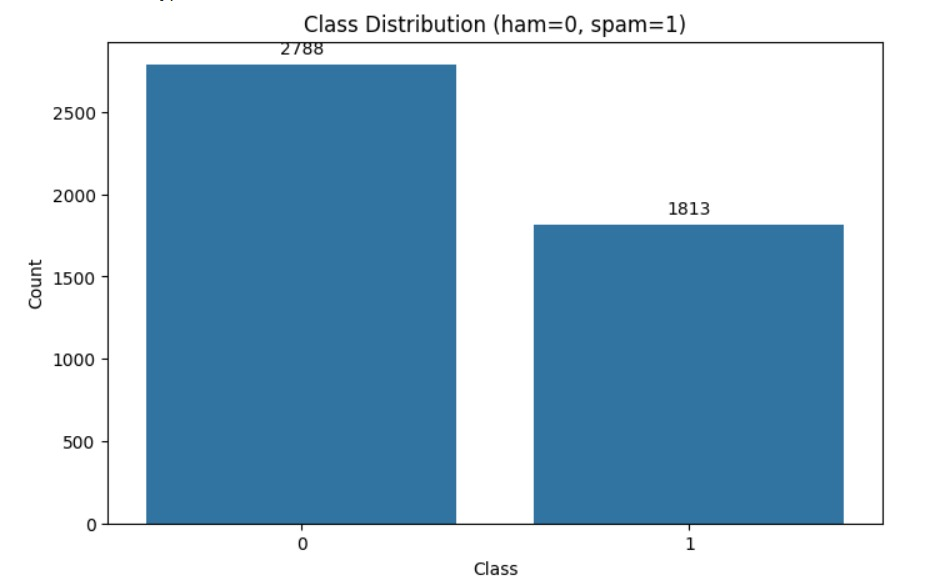
\includegraphics[width=0.45\textwidth]{class.jpeg}
\caption{Class distribution visualization}
\end{figure}

\subsection*{Top Features}
\begin{figure}[H]
\centering
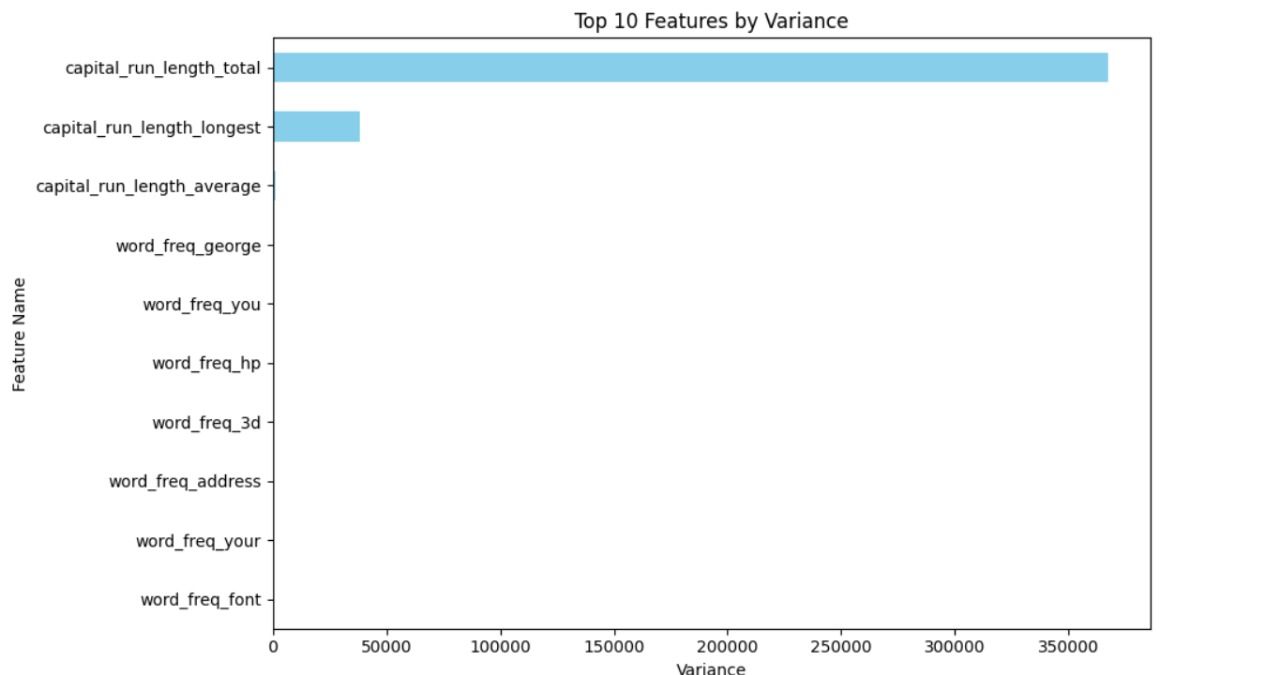
\includegraphics[width=0.45\textwidth]{top.jpeg}
\caption{Top 10 features by variance}
\end{figure}

\subsection*{Feature Distributions}
\begin{figure}[H]
\centering
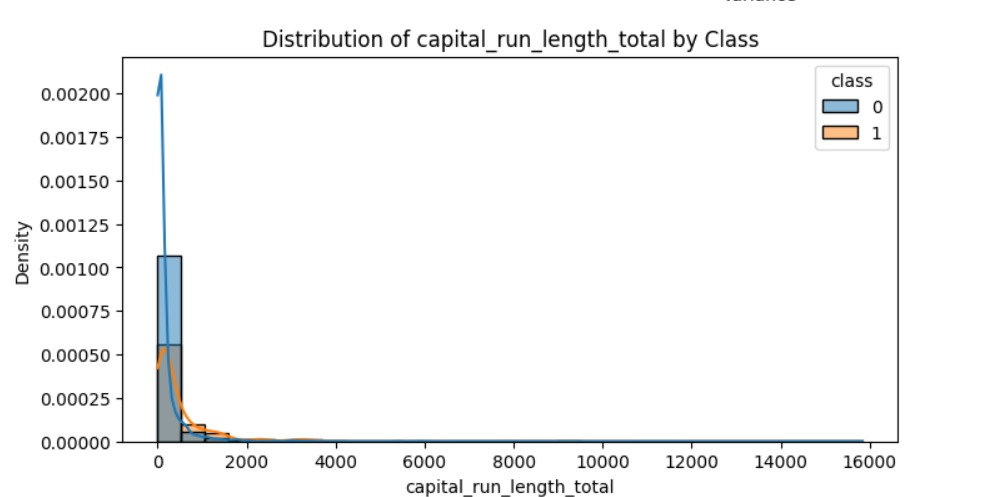
\includegraphics[width=0.45\textwidth]{feature.jpeg}
\caption{Feature distribution examples}
\end{figure}

\section*{CONFUSION MATRIX AND ROC CURVE}

\begin{figure}[H]
\centering
\begin{minipage}{0.45\textwidth}
\centering
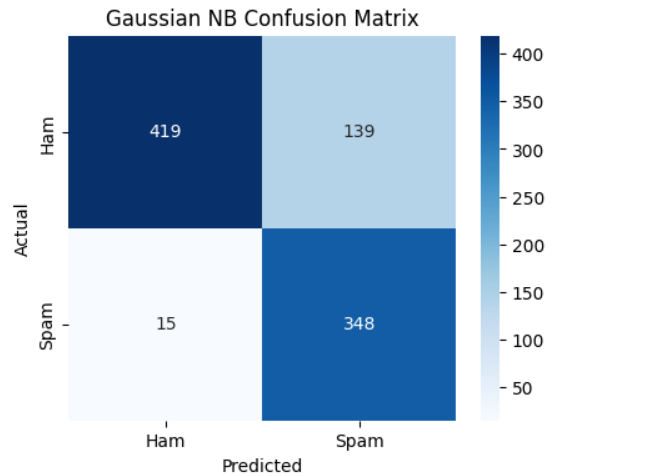
\includegraphics[width=\linewidth]{6.png}
\caption{Gaussian NB Confusion Matrix}
\end{minipage}
\hfill
\begin{minipage}{0.45\textwidth}
\centering
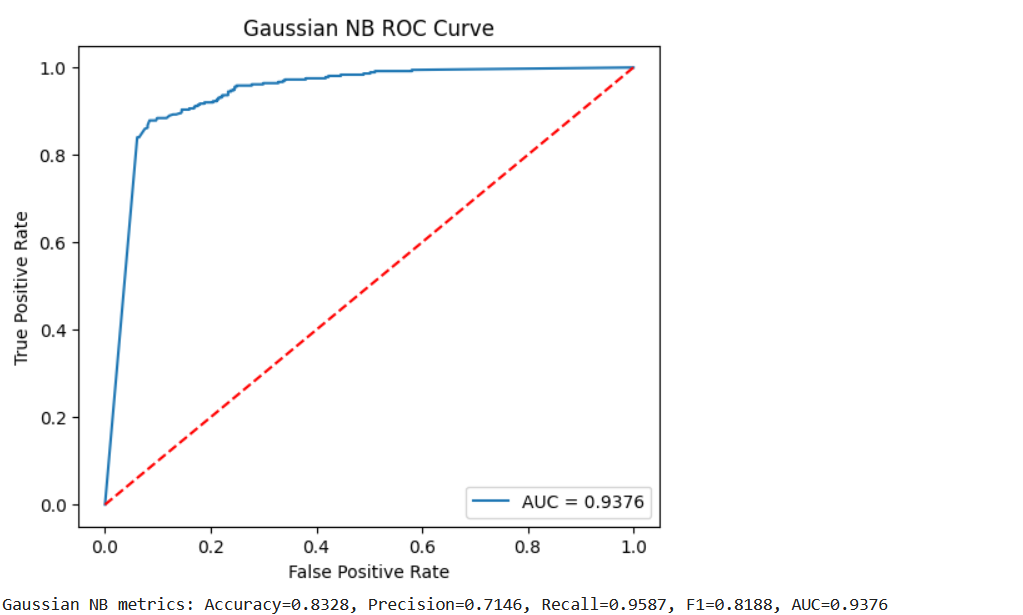
\includegraphics[width=\linewidth]{7.png}
\caption{Gaussian NB ROC Curve}
\end{minipage}
\end{figure}

\begin{figure}[H]
\centering
\begin{minipage}{0.45\textwidth}
\centering
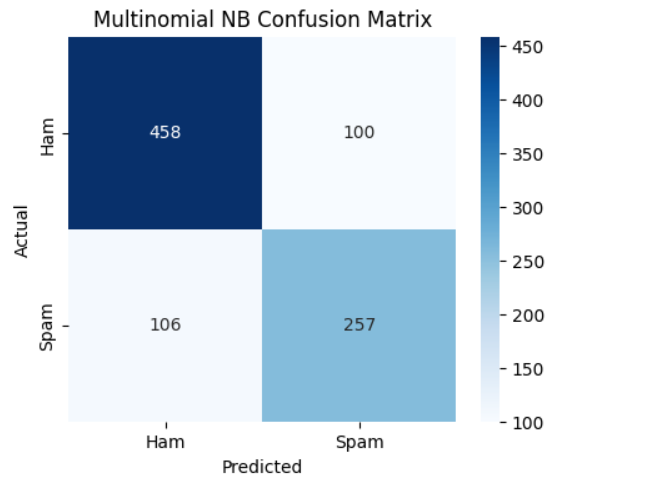
\includegraphics[width=\linewidth]{8.png}
\caption{Multinomial NB Confusion Matrix}
\end{minipage}
\hfill
\begin{minipage}{0.45\textwidth}
\centering
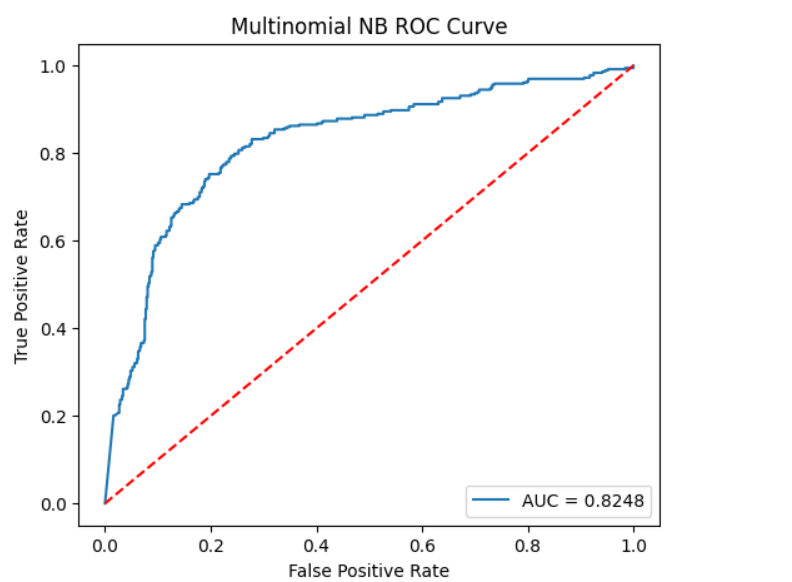
\includegraphics[width=\linewidth]{9.png}
\caption{Multinomial NB ROC Curve}
\end{minipage}
\end{figure}

\begin{figure}[H]
\centering
\begin{minipage}{0.45\textwidth}
\centering
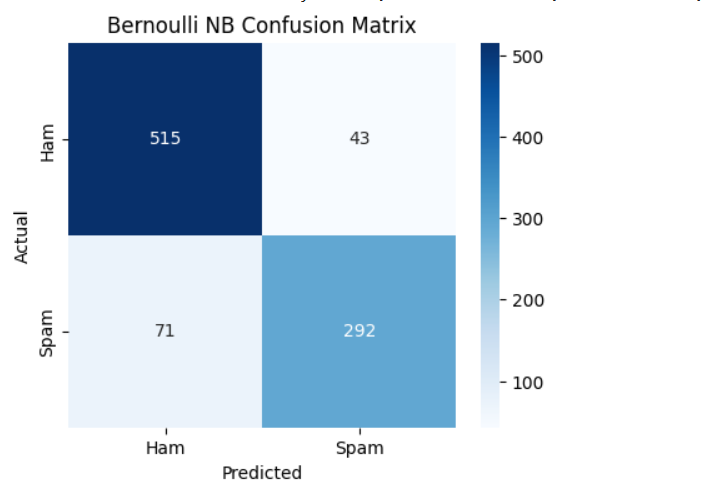
\includegraphics[width=\linewidth]{10.png}
\caption{Bernoulli NB Confusion Matrix}
\end{minipage}
\hfill
\begin{minipage}{0.45\textwidth}
\centering
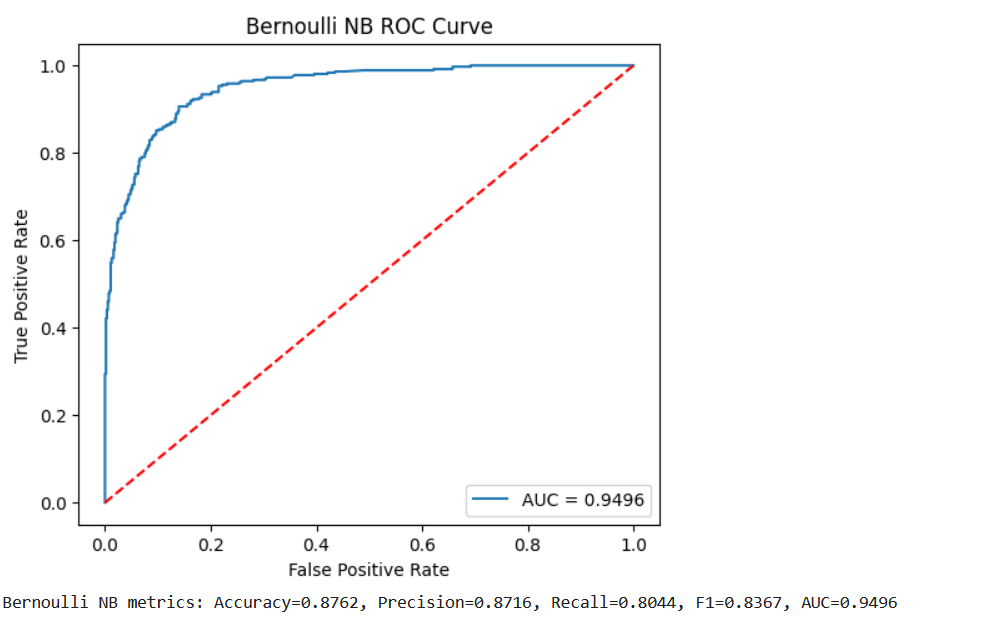
\includegraphics[width=\linewidth]{11.png}
\caption{Bernoulli NB ROC Curve}
\end{minipage}
\end{figure}

\begin{figure}[H]
\centering
\begin{minipage}{0.45\textwidth}
\centering
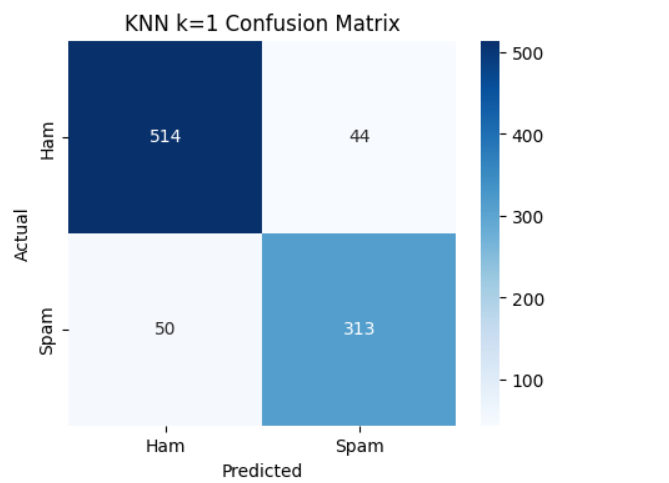
\includegraphics[width=\linewidth]{12.png}
\caption{KNN (k=1) Confusion Matrix}
\end{minipage}
\hfill
\begin{minipage}{0.45\textwidth}
\centering
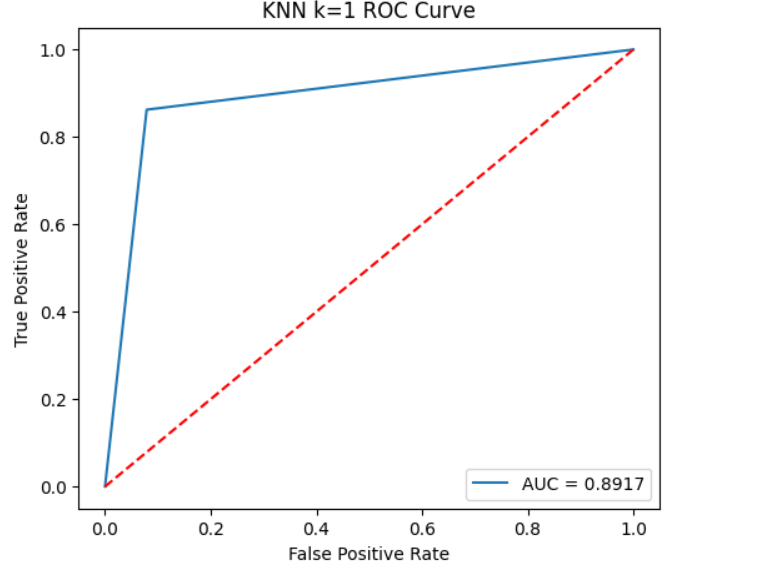
\includegraphics[width=\linewidth]{13.png}
\caption{KNN (k=1) ROC Curve}
\end{minipage}
\end{figure}

\begin{figure}[H]
\centering
\begin{minipage}{0.45\textwidth}
\centering
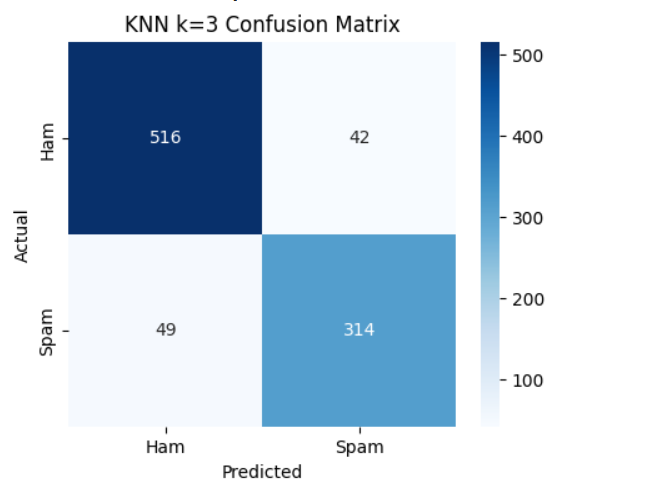
\includegraphics[width=\linewidth]{14.png}
\caption{KNN (k=3) Confusion Matrix}
\end{minipage}
\hfill
\begin{minipage}{0.45\textwidth}
\centering
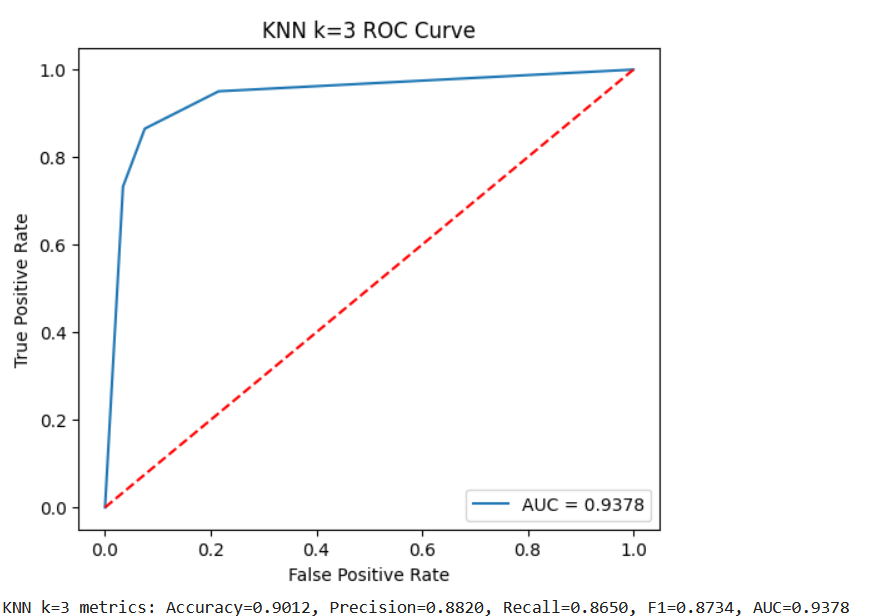
\includegraphics[width=\linewidth]{15.png}
\caption{KNN (k=3) ROC Curve}
\end{minipage}
\end{figure}

\begin{figure}[H]
\centering
\begin{minipage}{0.45\textwidth}
\centering
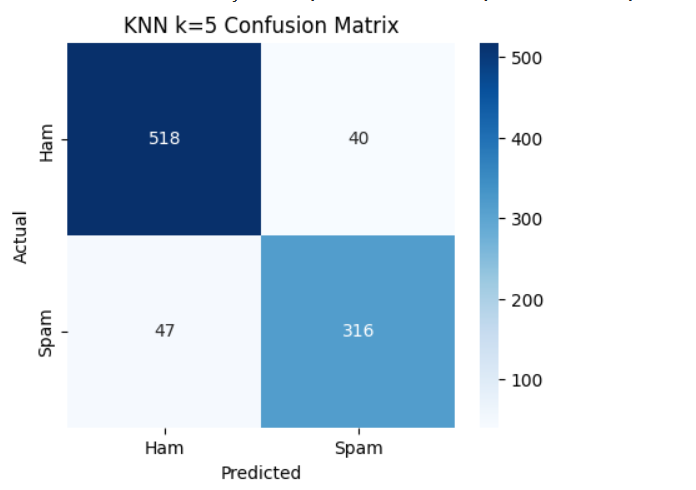
\includegraphics[width=\linewidth]{16.png}
\caption{KNN (k=5) Confusion Matrix}
\end{minipage}
\hfill
\begin{minipage}{0.45\textwidth}
\centering
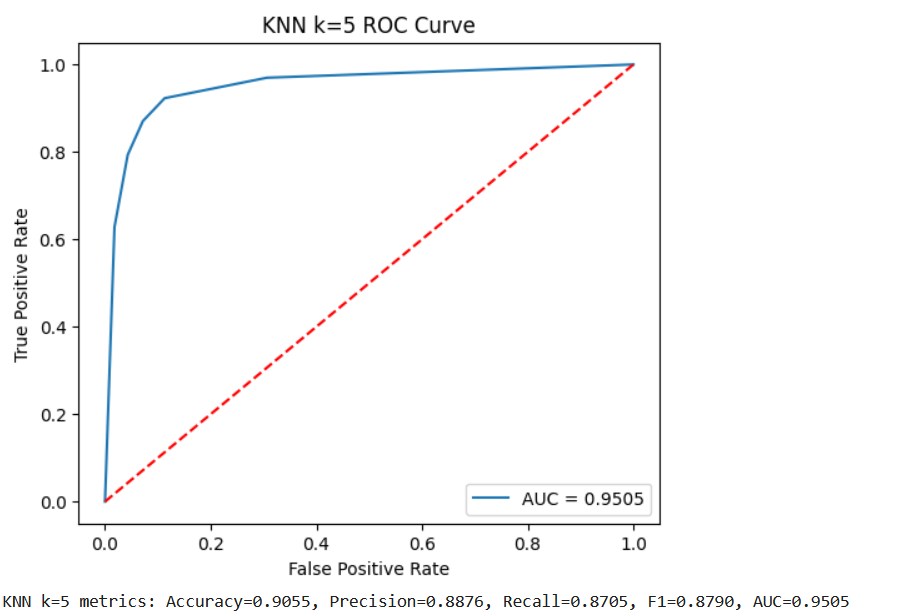
\includegraphics[width=\linewidth]{17.png}
\caption{KNN (k=5) ROC Curve}
\end{minipage}
\end{figure}

\begin{figure}[H]
\centering
\begin{minipage}{0.45\textwidth}
\centering
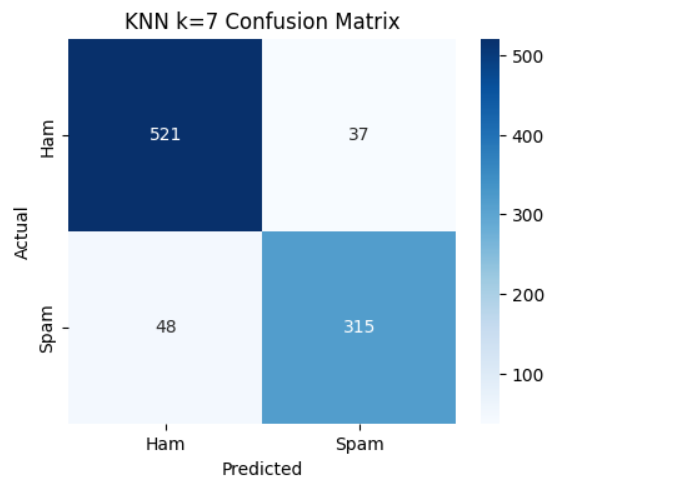
\includegraphics[width=\linewidth]{18.png}
\caption{KNN (k=7) Confusion Matrix}
\end{minipage}
\hfill
\begin{minipage}{0.45\textwidth}
\centering
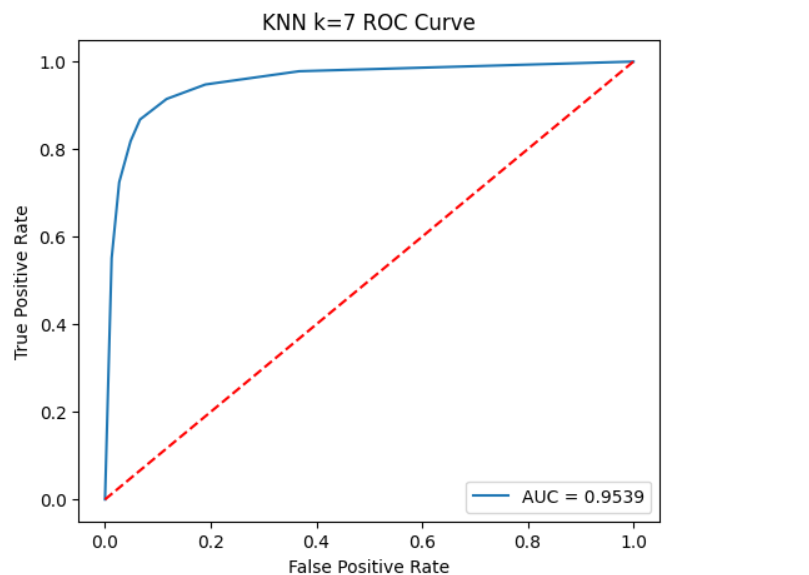
\includegraphics[width=\linewidth]{19.png}
\caption{KNN (k=7) ROC Curve}
\end{minipage}
\end{figure}

\begin{figure}[H]
\centering
\begin{minipage}{0.45\textwidth}
\centering
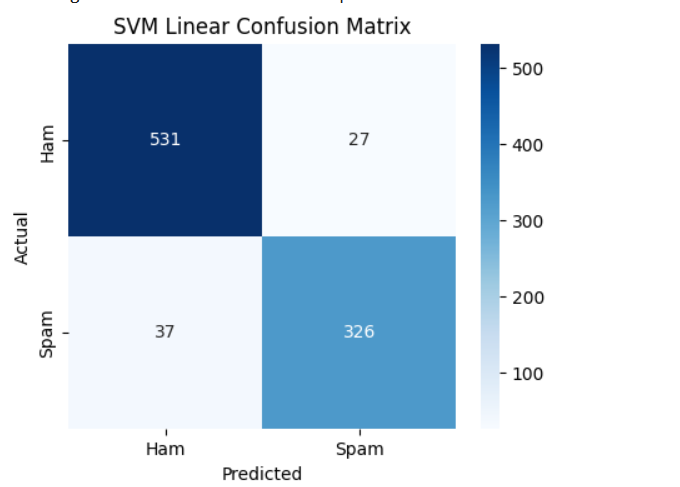
\includegraphics[width=\linewidth]{20.png}
\caption{SVM Linear Confusion Matrix}
\end{minipage}
\hfill
\begin{minipage}{0.45\textwidth}
\centering
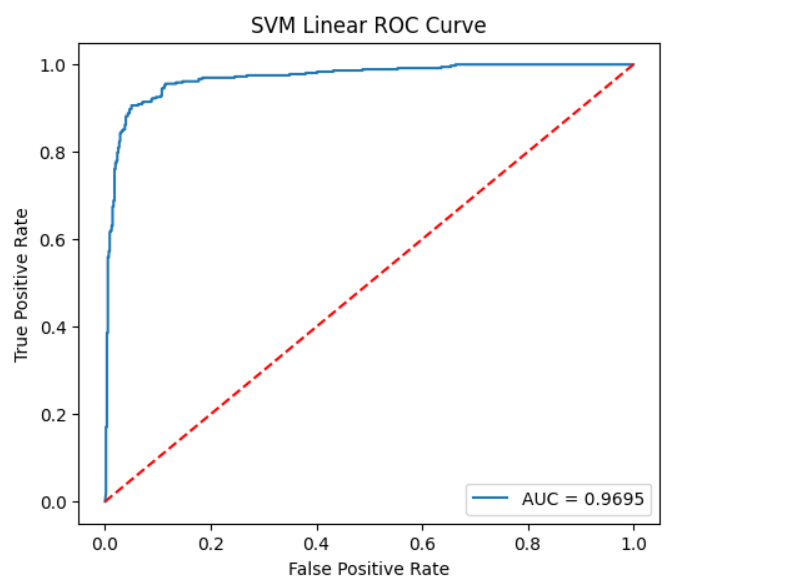
\includegraphics[width=\linewidth]{21.png}
\caption{SVM Linear ROC Curve}
\end{minipage}
\end{figure}

\begin{figure}[H]
\centering
\begin{minipage}{0.45\textwidth}
\centering
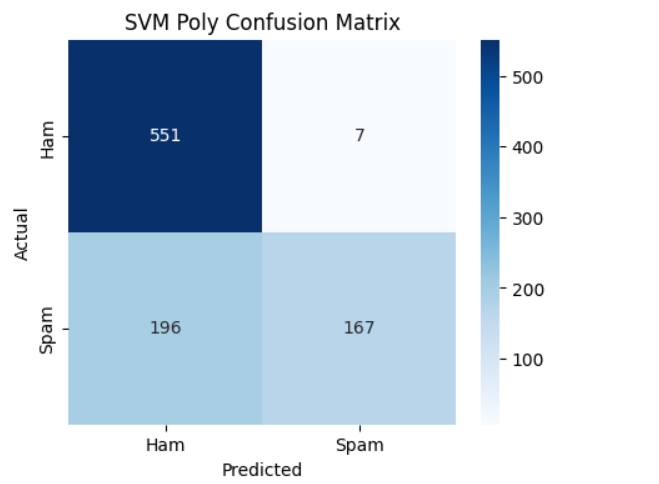
\includegraphics[width=\linewidth]{22.png}
\caption{SVM Polynomial Confusion Matrix}
\end{minipage}
\hfill
\begin{minipage}{0.45\textwidth}
\centering
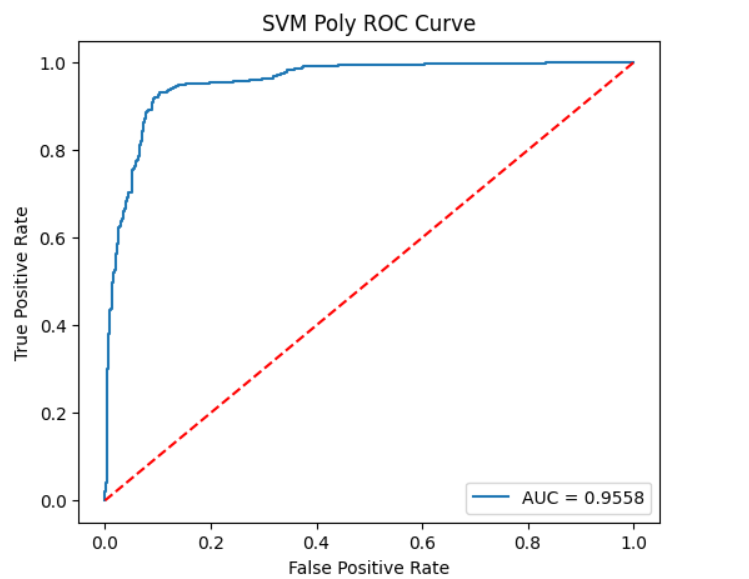
\includegraphics[width=\linewidth]{23.png}
\caption{SVM Polynomial ROC Curve}
\end{minipage}
\end{figure}

\begin{figure}[H]
\centering
\begin{minipage}{0.45\textwidth}
\centering
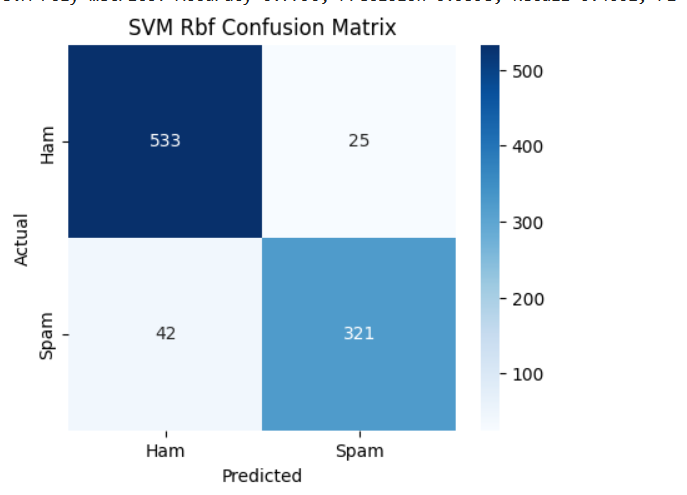
\includegraphics[width=\linewidth]{24.png}
\caption{SVM RBF Confusion Matrix}
\end{minipage}
\hfill
\begin{minipage}{0.45\textwidth}
\centering
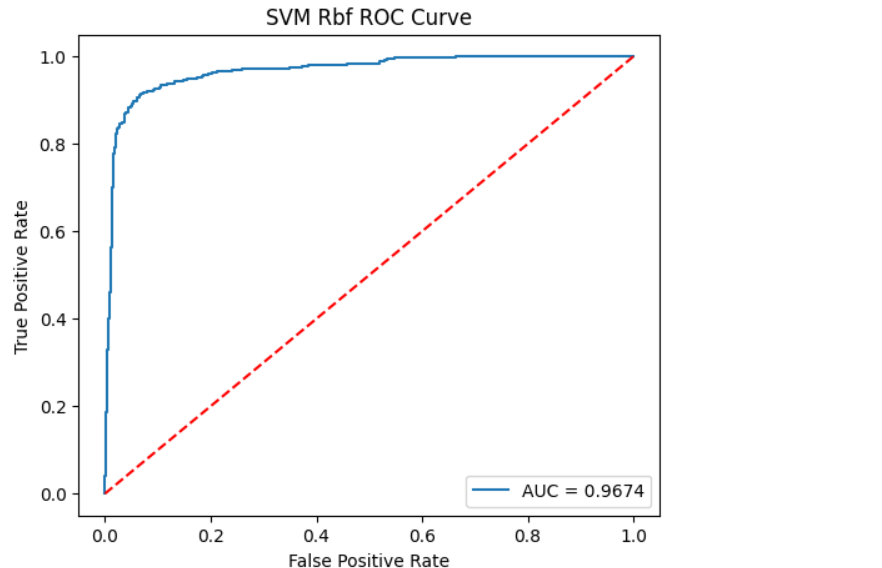
\includegraphics[width=\linewidth]{25.png}
\caption{SVM RBF ROC Curve}
\end{minipage}
\end{figure}

\begin{figure}[H]
\centering
\begin{minipage}{0.45\textwidth}
\centering
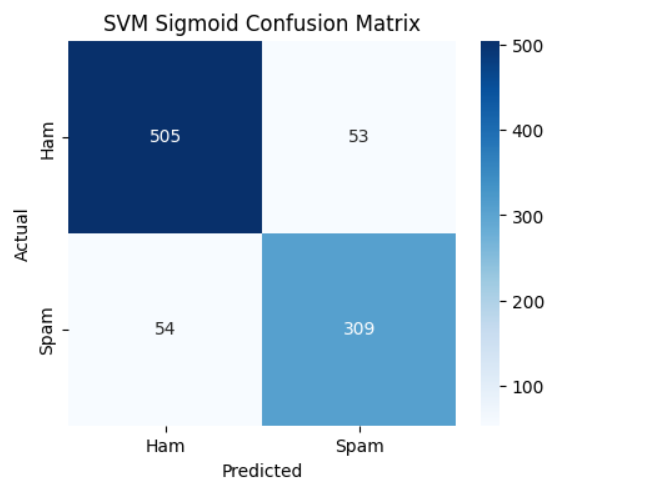
\includegraphics[width=\linewidth]{26.png}
\caption{SVM Sigmoid Confusion Matrix}
\end{minipage}
\hfill
\begin{minipage}{0.45\textwidth}
\centering
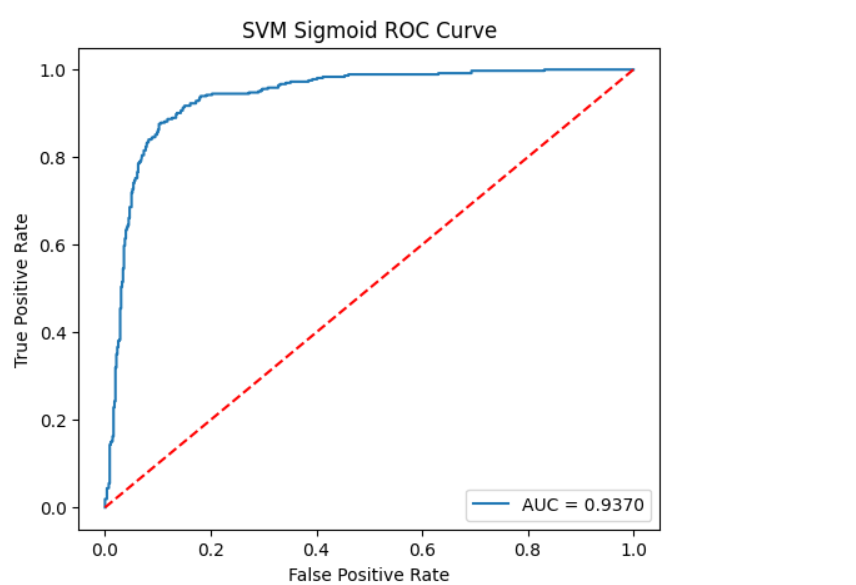
\includegraphics[width=\linewidth]{27.png}
\caption{SVM Sigmoid ROC Curve}
\end{minipage}
\end{figure}

\section*{RESULT SUMMARY TABLES}

\subsection*{Table 1: Naïve Bayes Variant Comparison}
\begin{center}
\begin{tabular}{lccccc}
\toprule
\textbf{Variant} & \textbf{Accuracy} & \textbf{Precision} & \textbf{Recall} & \textbf{F1 Score} & \textbf{AUC} \\
\midrule
Gaussian NB & 0.8328 & 0.7146 & 0.9587 & 0.8188 & 0.9376 \\
Multinomial NB & 0.7763 & 0.7199 & 0.7080 & 0.7139 & 0.8248 \\
Bernoulli NB & 0.8762 & 0.8716 & 0.8044 & 0.8367 & 0.9496 \\
\bottomrule
\end{tabular}
\end{center}

\subsection*{Table 2: KNN Performance for Different $k$ Values}
\begin{center}
\begin{tabular}{lccccc}
\toprule
\textbf{k} & \textbf{Accuracy} & \textbf{Precision} & \textbf{Recall} & \textbf{F1 Score} & \textbf{AUC} \\
\midrule
1 & 0.8979 & 0.8768 & 0.8623 & 0.8694 & 0.8917 \\
3 & 0.9012 & 0.8820 & 0.8650 & 0.8734 & 0.9378 \\
5 & 0.9055 & 0.8876 & 0.8705 & 0.8790 & 0.9505 \\
7 & 0.9077 & 0.8949 & 0.8678 & 0.8811 & 0.9539 \\
\bottomrule
\end{tabular}
\end{center}

\subsection*{Table 3: KNN Comparison: KDTree vs BallTree}
\begin{center}
\begin{tabular}{lcc}
\toprule
\textbf{Metric} & \textbf{KDTree} & \textbf{BallTree} \\
\midrule
Accuracy & 0.9055 & 0.9055 \\
Precision & 0.8876 & 0.8876 \\
Recall & 0.8705 & 0.8705 \\
F1 Score & 0.8790 & 0.8790 \\
Training Time (s) & 0.0343 & 0.0124 \\
\bottomrule
\end{tabular}
\end{center}


\subsection*{Table 4: SVM Performance with Different Kernels and Hyperparameters}
\begin{center}
\begin{tabular}{l l c c c}
\toprule
\textbf{Kernel} & \textbf{Hyperparameters} & \textbf{Accuracy} & \textbf{F1 Score} & \textbf{Training Time (s)} \\
\midrule
Linear & C=0.1 & 0.9245 & 0.9083 & 1.3663 \\
Linear & C=1.0 & 0.9296 & 0.9106 & 2.8080 \\
Linear & C=10.0 & 0.9293 & 0.9063 & 14.2990 \\
Poly & C=0.1, degree=2, gamma=scale & 0.7101 & 0.4990 & 4.6430 \\
Poly & C=0.1, degree=2, gamma=auto & 0.7122 & 0.5081 & 4.7247 \\
Poly & C=0.1, degree=3, gamma=scale & 0.6845 & 0.3921 & 3.5441 \\
Poly & C=0.1, degree=3, gamma=auto & 0.6859 & 0.3956 & 4.5605 \\
Poly & C=1.0, degree=2, gamma=scale & 0.8334 & 0.7718 & 2.7677 \\
Poly & C=1.0, degree=2, gamma=auto & 0.8348 & 0.7805 & 2.7534 \\
Poly & C=1.0, degree=3, gamma=scale & 0.7663 & 0.6220 & 3.3830 \\
Poly & C=1.0, degree=3, gamma=auto & 0.7685 & 0.6422 & 3.9291 \\
RBF & C=0.1, gamma=scale & 0.9062 & 0.8835 & 2.7757 \\
RBF & C=0.1, gamma=auto & 0.9054 & 0.8851 & 2.8310 \\
RBF & C=1.0, gamma=scale & 0.9340 & 0.9055 & 1.8260 \\
RBF & C=1.0, gamma=auto & 0.9340 & 0.9055 & 2.8488 \\
RBF & C=10.0, gamma=scale & 0.9332 & 0.9001 & 1.7754 \\
RBF & C=10.0, gamma=auto & 0.9332 & 0.9001 & 1.6441 \\
Sigmoid & C=0.1, gamma=scale & 0.8910 & 0.8530 & 2.9397 \\
Sigmoid & C=0.1, gamma=auto & 0.8916 & 0.8547 & 2.9691 \\
Sigmoid & C=1.0, gamma=scale & 0.8804 & 0.8524 & 2.6172 \\
Sigmoid & C=1.0, gamma=auto & 0.8804 & 0.8508 & 2.3010 \\
\bottomrule
\end{tabular}
\end{center}

\subsection*{Table 5: Cross-Validation Scores for Each Model (K=5)}
\begin{center}
\begin{tabular}{lccc}
\toprule
\textbf{Fold} & \textbf{Naïve Bayes (Bernoulli)} & \textbf{KNN (k=5)} & \textbf{SVM (RBF)} \\
\midrule
Fold 1 & 0.8806 & 0.9034 & 0.9349 \\
Fold 2 & 0.8902 & 0.9174 & 0.9337 \\
Fold 3 & 0.8837 & 0.9359 & 0.9228 \\
Fold 4 & 0.8870 & 0.9141 & 0.9359 \\
Fold 5 & 0.8902 & 0.9152 & 0.9304 \\
\textbf{Average} & \textbf{0.8863} & \textbf{0.9172} & \textbf{0.9315} \\
\bottomrule
\end{tabular}
\end{center}

\section*{Learning Outcome (observation)}
\begin{itemize}
  \item \textbf{Best Classifier:} SVM with RBF kernel had the highest average accuracy (93.15\%).
  \item \textbf{Best Naïve Bayes:} Bernoulli Naïve Bayes performed best among NB variants.
  \item \textbf{KNN Variability:} Accuracy increased with $k$, peaking at $k=7$. Both KDTree and BallTree yielded same metrics but BallTree had faster training.
  \item \textbf{SVM Insights:} RBF and Linear kernels outperformed Poly and Sigmoid. Hyperparameter tuning further improved performance.
\end{itemize}

\end{document}
